\chapter{Part B: Data Analysis}

\section{Data pre-processing and experimental setup}

We combined two Equinox datasets containing change metrics and CK/OO metrics and used the class identifier \texttt{classname} as the join key. Defect-related metadata columns were removed from the feature set, while \texttt{bugs} was retained as the target variable.

We merged the two datasets using a one-to-one inner join on \texttt{classname}. After merging, all feature columns, as well as the target, were converted to numeric values. The final dataset contains \textbf{324 classes}, \textbf{32 features}, and one target variable.

The dataset was split into a training set (67\%) and a test set (33\%). To preserve the distribution of bug counts, we used stratified random sampling based on the predefined bug-count bins (0, 1--2, 3--5, 6+). The stratification variable was used only for splitting and removed afterwards.

The resulting training and test sets were saved and used consistently in all analyses. Models were selected on the training set and the final selected model was evaluated on the test set.

\subsection{Data Analysis}

Before training our Poisson and logistic regression models, we first investigate the distribution of the data.

As a first step, we plot the histogram of the 32 features that we use in Figure~\ref{fig:feature_histogram_raw}. While we only display the marginal distributions of the features, and therefore omit the joint interaction between multiple features, plotting the joint interaction would require 512 plots, which, for the scope of this task, is too much to look at.

Figure~\ref{fig:feature_histogram_raw} clearly shows that most of the data are not only skewed to the left, i.e., have most of their value close to zero with heavy tails containing high values, but we also remark that the range of certain variables is extremely large (e.g. \texttt{numberOfLinesOfCode} which spans the range of around 0--1500).

% To counteract this effect, we propose to first transform the data 

While the skewness of the response variable is not an issue, as we use Poisson regression, which can handle skewed data, and logistic regression for the binary case, we argue that the skewness in the features might impact the model negatively.
Therefore, we propose to transform the 32 features into the log-domain, which should reduce the effect of the skewness.

Finally, to make the training of the models easier, we normalize every feature such that they have a mean of zero and a standard deviation of 1. While this hinders slightly the interpretation of the learned parameter $\beta$, we remark that by using the inverse of the normalization used on the features, we can give meaning to the learned parameters again.

We plot the distribution of the log-transformed and normalized features in Figure~\ref{fig:feature_histogram_log_transformed}. While we observe that many features remain skewed to the left, we also observe that the values of the features are more evenly distributed, with many features almost containing a gaussian bell shape (e.g. \texttt{avgCodeChrunUntil}). 

\begin{figure}[t]
    \centering
    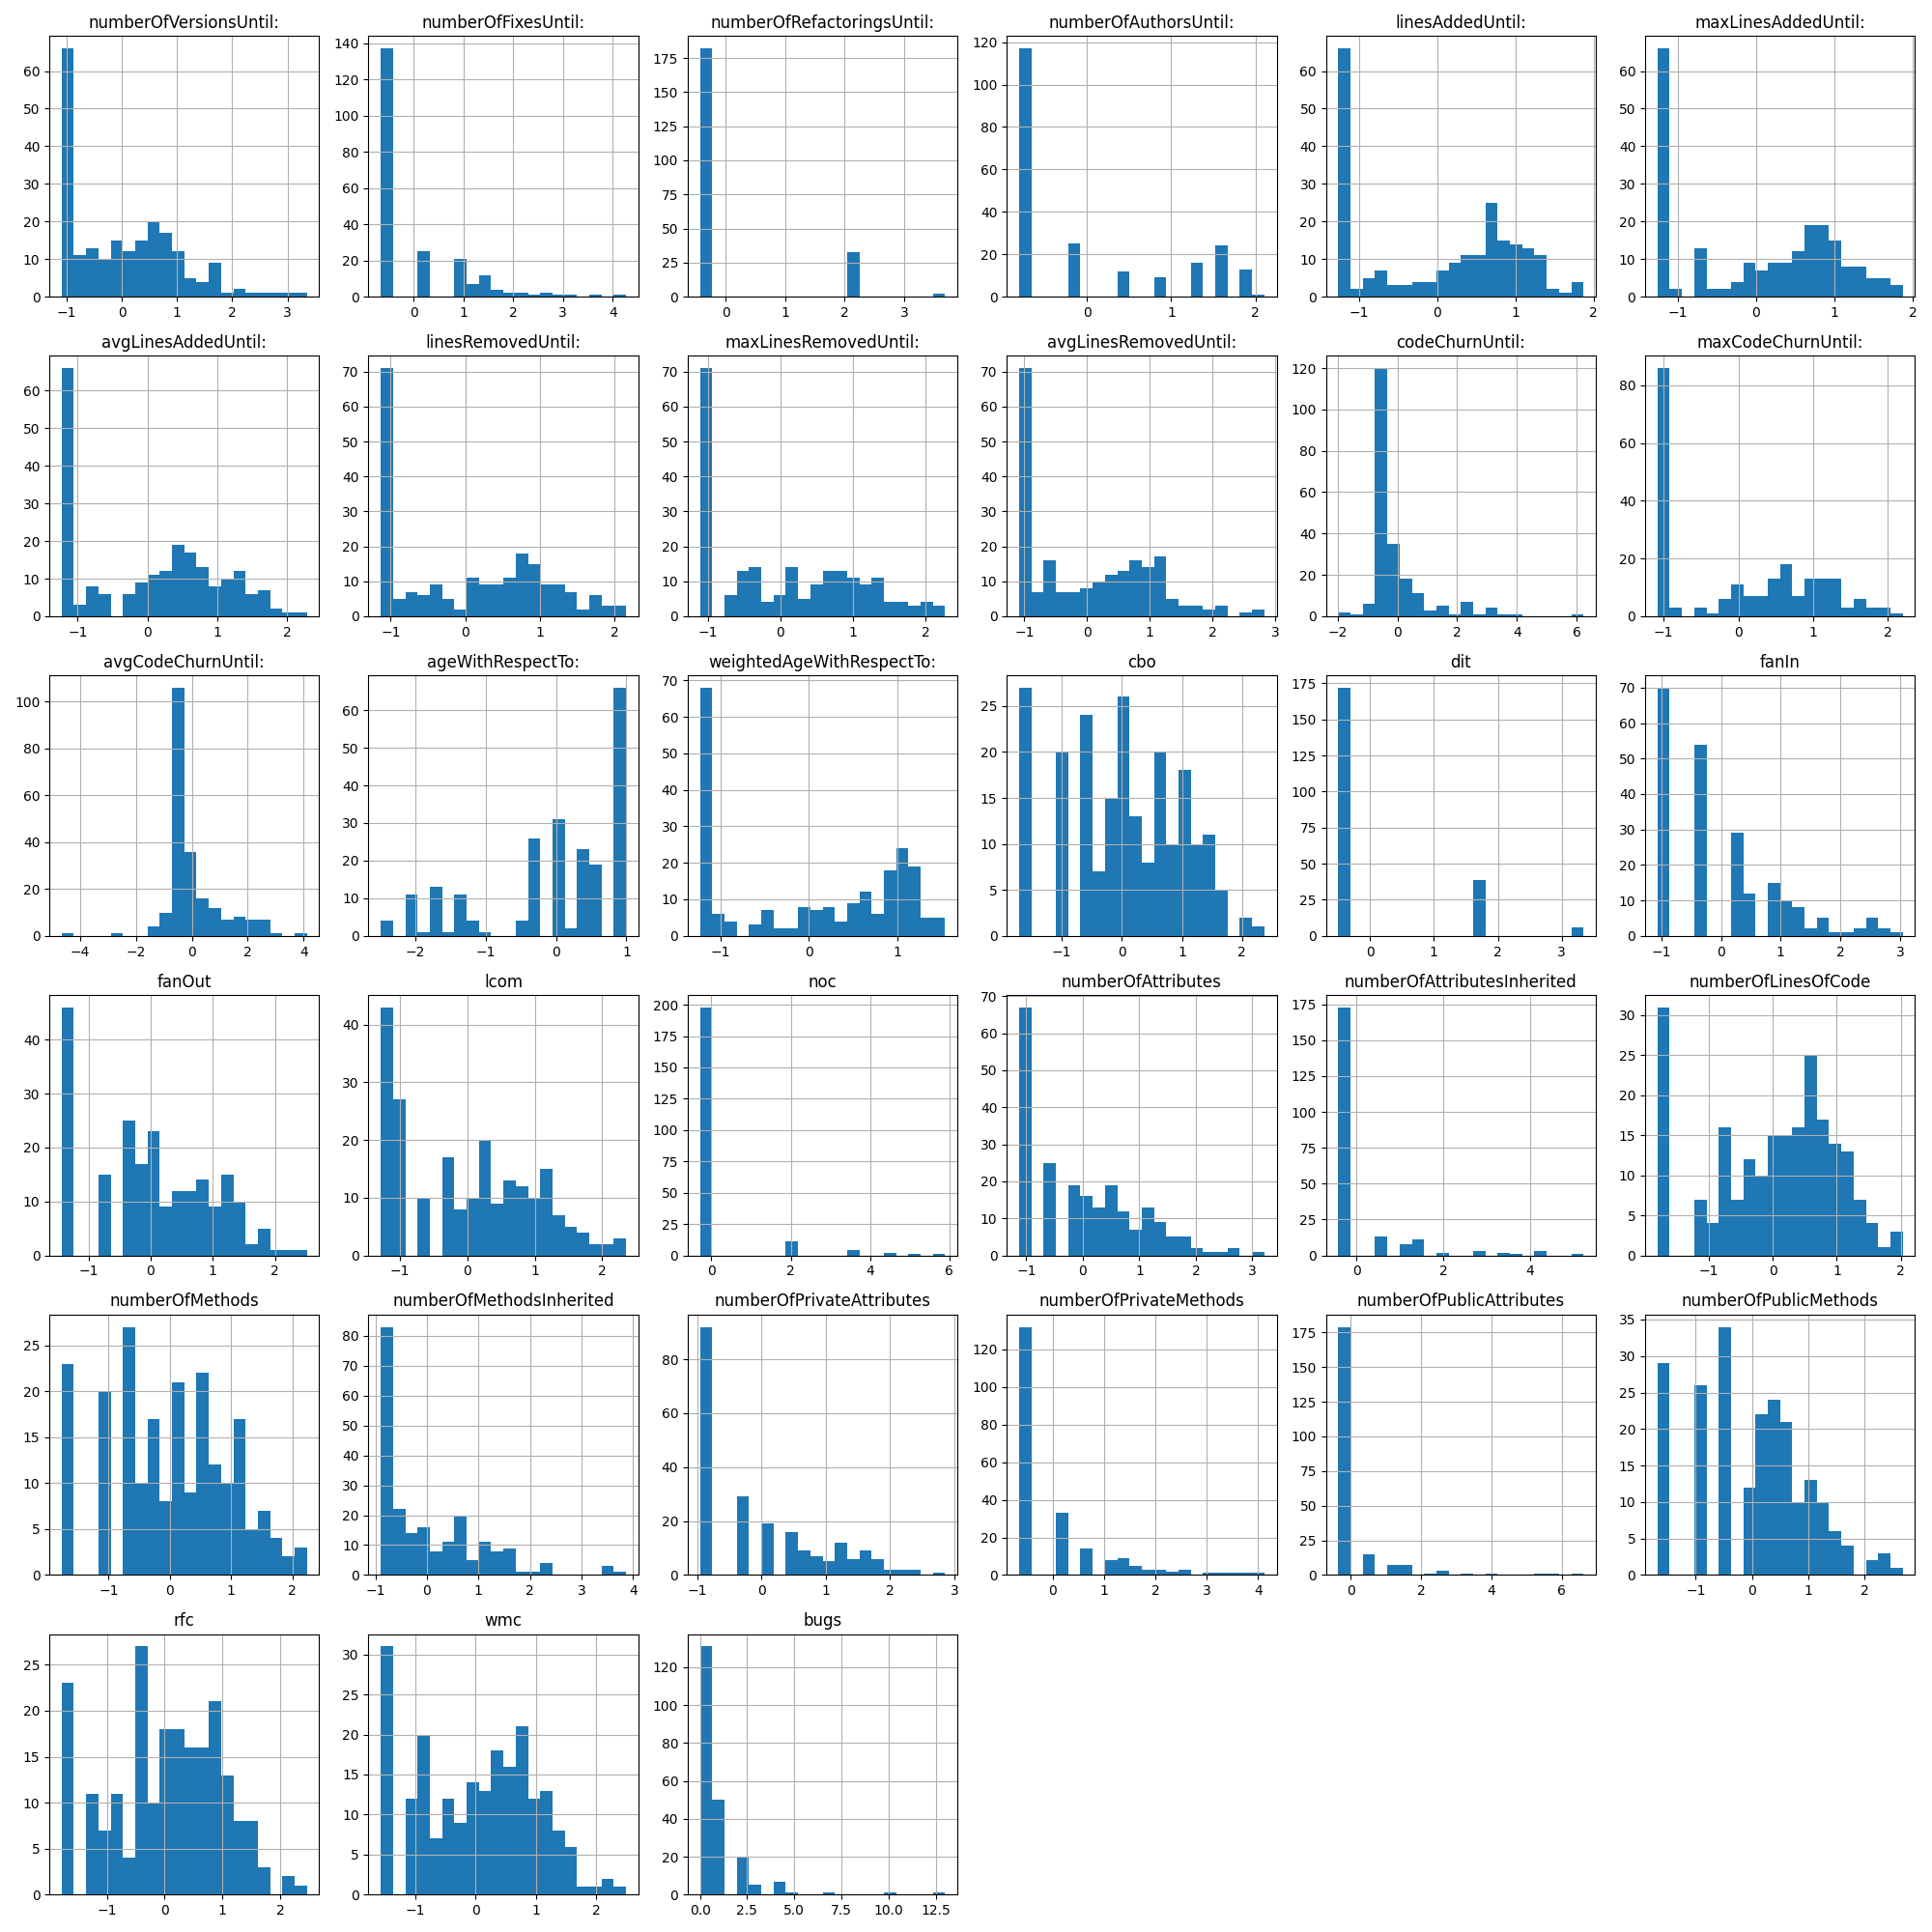
\includegraphics[width=0.75\linewidth]{extra_plots/raw_feature_histograms_log_and_normalized.png}
    \caption{Histograms of the 32 features after transforming them into the log domain and normalizing them.}
    \label{fig:feature_histogram_log_transformed}
\end{figure}

As the log-transformation might have destroyed the (linear) relationship of certain variables --- especially if it is with the response variable --- we will compare performance of the log-transformed and normalized data to the just normalized data.

Note that to ensure a valid log-transformation, we added a constant to each of the features, to ensure that each feature is greater than zero. This is part of our log-transform step.

\section{Poisson regression}

\subsection{Stepwise model selection}
\label{sec:poisson_stepwise}
We use Poisson regression to model the number of bugs for each function.
To find the best set of features to use for the Poisson regression,
% Since the response variable is count data, a generalized linear model with Poisson family and log link was used. 
we performed model selection using both forward and backward stepwise selection, starting from a model with only an intercept.

To find the best model from the training features alone, we scored each found model using both AIC and BIC, as we are also interested in understanding when one is better than the other.

\begin{figure}[t]
    \centering
    {\textbf{Normalized} Data} \\
    \subfloat[Using \textbf{AIC}.]{
        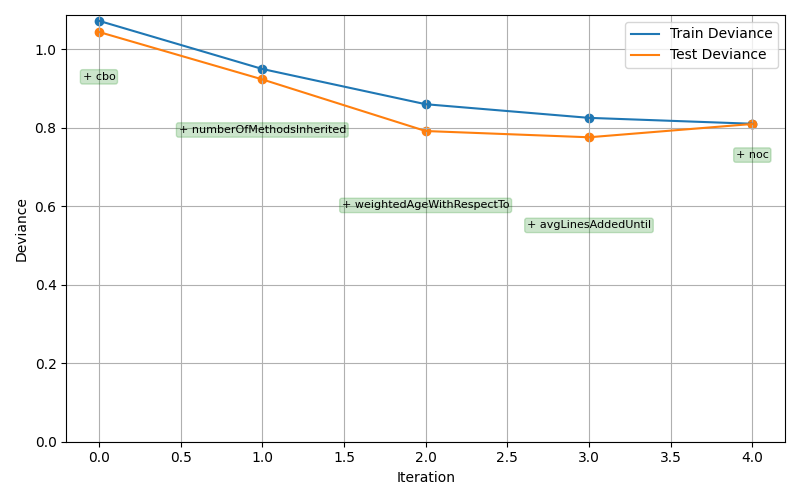
\includegraphics[width=0.45\linewidth]{extra_plots/poisson_regression_stepwise_deviance_history_aic.png}
    }
    \hfill
    \subfloat[Using \textbf{BIC}.]{
        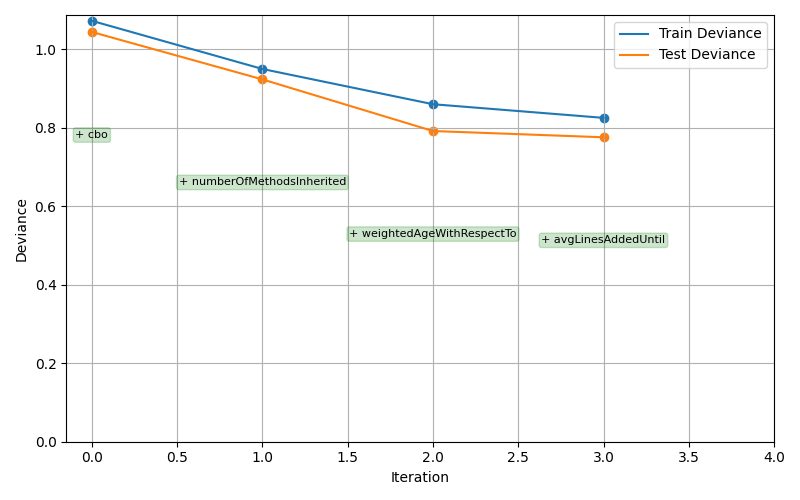
\includegraphics[width=0.45\linewidth]{extra_plots/poisson_regression_stepwise_deviance_history_bic.png}
    }
    \caption{Train and test deviance of the Poisson regression when using stepwise model selection when using the normalized featured. Note that the green boxes starts with + denote which feature has been added to the model.}
    \label{fig:deviance_normalized}
\end{figure}


\begin{figure}[t]
    \centering
    {\textbf{Log-transformed \& Normalized} Data} \\
    \subfloat[Using \textbf{AIC}.]{
        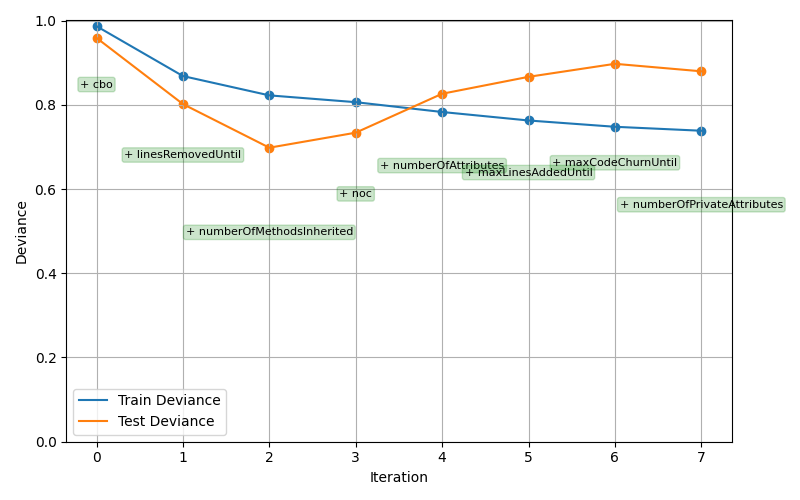
\includegraphics[width=0.45\linewidth]{extra_plots/poisson_regression_stepwise_deviance_history_aic_log.png}
    }
    \hfill
    \subfloat[Using \textbf{BIC}.]{
        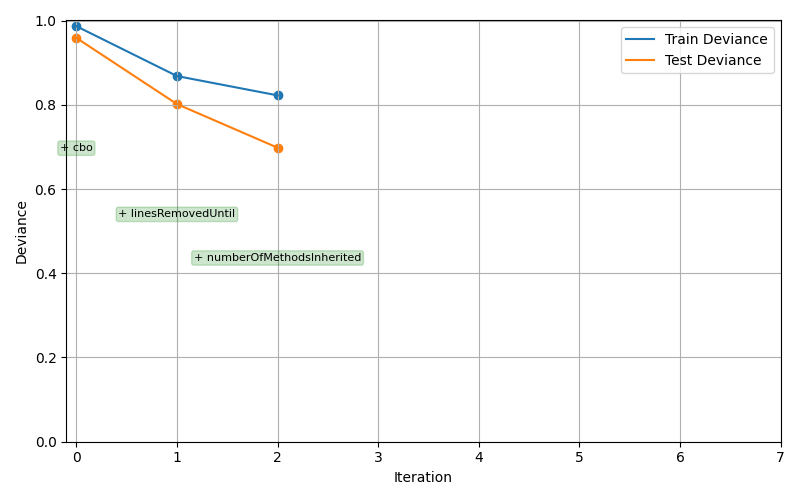
\includegraphics[width=0.45\linewidth]{extra_plots/poisson_regression_stepwise_deviance_history_bic_log.png}
    }
    \caption{Train and test deviance of the Poisson regression when using stepwise model selection when using the log-transformed and normalized featured. Note that the green boxes starts with + denote which feature has been added to the model.}
    \label{fig:deviance_log_transformed_and_normalized}
    % \label{stepwise vs LASSO}
\end{figure}


\textbf{Normalized Data.}
Let us first look at the results from the Poisson regression models found using stepwise model selection. 
In Figure~\ref{fig:deviance_normalized}, we have plotted the train and test poisson-deviation at each step, while using the AIC and BIC scores to estimate when to stop the search. We report on the final mean Poisson deviance in Table~\ref{tab:mean_poisson_deviation_poisson_regression_step_search}.

First, when using AIC, we find a model using 5 features, namely \texttt{cbo}, \texttt{numberOfMethodsInherited}, \\\texttt{weightedAgeWithRespectTo}, \texttt{avgLinesAddedUntil}, and \texttt{noc}.
Interestingly, while the Poisson deviance decreases with each feature that is being added, we observe that adding the \texttt{noc} features makes the test deviance increase, while the train deviance decreases.
This is a sign of overfitting.

Interestingly, when using BIC to score the models, we observe that the same features are being added in the same order. However, when adding a fifth feature, including \texttt{noc}, the BIC score increases, and therefore the search stops. 

\textbf{Log-Transformed and Normalized Data.}
We run the same code on the data we transformed to the log space. We plot the train and test mean Poisson deviance in Figure~\ref{fig:deviance_log_transformed_and_normalized} and report on the final mean Poisson deviance in Table~\ref{tab:mean_poisson_deviation_poisson_regression_step_search}.

First, we remark that, compared to the normalized data, using AIC for scoring the search finds 7 features, whereas when using BIC, only 3 features are found.

Similarly as for the just normalized data, BIC stops the search as soon as the Poisson deviance of the test set increases, while finding the same sets of features.

Interestingly, we remark that first transforming the data to the log domain uncovers new relationships. This can be seen from the first model from both Figure~\ref{fig:deviance_normalized} and Figure~\ref{fig:deviance_log_transformed_and_normalized}, which only consists of the \texttt{cbo} feature and an intercept. 
Whereas for the just normalized data, the train and test deviance is above 1, when using the log-transformed data, the mean Poisson deviance is bellow 1 for both the train and test set.

This clearly shows that transforming the features to the log space allows the linear relationship to explain more of the variance, and therefore have better predictions.


% Train deviance: 0.8256935176391517
% Test deviance: 0.7761751965293804
% Train deviance: 0.7383483742906413
% Test deviance: 0.8794590092835627
% Train deviance: 0.8223124733984547
% Test deviance: 0.6980782248498346
\begin{table}[tbp]
    \centering
    \begin{tabular}{ll|cc}
         \toprule
         Search Score & Dataset & Train Deviation ($\downarrow$) & Test ($\downarrow$)  \\
         % \toprule
         \midrule
         \multirow{2}{*}{AIC} & Normalized & $0.81064$ & $0.81010$ \\
         &Log-Transformed \& Normalized & $\textbf{0.73834}$ & $0.87946$ \\
         \midrule
         \multirow{2}{*}{BIC} & Normalized & $ 0.82569$ & $0.77617$ \\
         &Log-Transformed \& Normalized & ${0.82231}$ & $\mathbf{0.69807}$ \\
         \bottomrule
    \end{tabular}
    \caption{The mean Poisson deviation values for the best \textbf{Poisson regression model} obtained using \textbf{Stepwise model search} for the different datasets. We highlight in bold the best value of the table for each of the data splits.}
    \label{tab:mean_poisson_deviation_poisson_regression_step_search}
\end{table}


\textbf{Analysis of the Parameters.}
Before looking at the Logistic regression, let us first investigate the values of the found parameters.
From the lecture, we know that increasing the features of a sample $x\in \mathbb{R}^D$ by $\delta\in\mathbb{R}^D$ results in
\begin{equation}
    \frac{\mathbb{E}[y\mid x+\delta]}{\mathbb{E}[y\mid x]} = \exp(\beta \cdot \delta)\;. 
    \label{eq:increase_parameter}
\end{equation}
We can easily understand the impact of each parameter on the prediction by constructing $\delta$ as follows: Let us investigate the increase of the raw feature by one unit. We can construct such a $\delta_i$ for each feature as follows:
\begin{equation*}
    \delta_i = \frac{1}{\sigma_i}
\end{equation*}
as we have 
{
\allowdisplaybreaks
\begin{align*}
    \mathrm{Normalized}(x) + \delta_i &= \frac{x-\mu}{\sigma} + (0, \dots, \underbrace{\frac{1}{\sigma_i}}_i, \dots, 0) \\
    &= \frac{x-\mu}{\sigma} + \frac{1}{\sigma}(0, \dots, \underbrace{1}_i, \dots, 0) \\
    &= \frac{x-\mu}{\sigma} + \frac{1}{\sigma}\delta \\
    &= \frac{x -\mu + \delta}{\sigma} \\
    &= \mathrm{Normalize}(x+\delta)
\end{align*}
}
with $\delta$ denoting a one hot vector at the index of the feature of interest.

It is important to note that we are unable to perform such a simple analysis of the coefficient for the log-transformed data. This is because $\log(x+1) \neq \log(x)+\log(1)$, and the increase of the a feature by one changes the prediction depending on $x$. 

While we could compute the expected change in prediction by computing the probability of observing each value of a feature based on the data, we believe that the high-variance induced by the estimated probability would render any analysis meaningless.

Therefore, we only report on the influence of the coefficient for the normalized features. 

% Note that for the log-transform, we have
% \begin{equation*}
%     \delta_i = \frac{\log(1+c)}{\sigma_i}
% \end{equation*}
% where $c\in \mathbb{R}$ denote the constant added to each feature to ensure that each feature is positive.
% The final model selected by stepwise regression includes the following five predictors:
% \[
% \text{bugs} \sim \textit{cbo} + \textit{numberOfMethodsInherited} + \textit{weightedAgeWithRespectTo}
% + \textit{avgLinesAddedUntil} + \textit{noc}
% \]

% Therefore, combining 

% We have the following values for the parameters of the models:
% \begin{table}[]
%     \centering
%     \begin{tabular}{l|c c c c}
%          \textbf{Variable} & \textbf{Coefficient} & $\frac{\mathbb{E}[y\mid x+\delta_i]}{\mathbb{E}[y\mid x]}$  & \textbf{p-value} & \textbf{95\% CI} \\
%          \toprule
%          Intercept & $0$ & - & $0$ & $[0, 1]$ \\
%          \texttt{cbo} & $-0.2$
%     \end{tabular}
%     \caption{Caption}
%     \label{tab:placeholder}
% \end{table}


\begin{table}[htbp]
    \centering
    \begin{tabular}{l c c c c}
        \toprule
        \textbf{Variable} & \textbf{Coefficient} & $\frac{\mathbb{E}[y\mid x+\delta_i]}{\mathbb{E}[y\mid x]}$ & \textbf{p-value} & \textbf{95\% CI} \\
        \midrule
        Intercept * & $-0.800$ & -- & $<0.001$ & $[-1.017,\,-0.583]$ \\
        \texttt{cbo} * & $0.496$ & $0.929$ & $<0.001$ & $[0.419,\,0.572]$ \\
        \texttt{numberOfMethodsInherited} * & $0.236$ & $1.036$ & $<0.001$ & $[0.148,\,0.324]$ \\
        \texttt{weightedAgeWithRespectTo:} * & $0.392$ & $1.007$ & $<0.001$ & $[0.245,\,0.538]$ \\
        \texttt{avgLinesAddedUntil:} * & $0.205$ & $1.016$ & $0.002$ & $[0.075,\,0.335]$ \\
        \texttt{noc} & $0.109$ & $1.401$ & $0.052$ & $[-0.001,\,0.219]$ \\
        \bottomrule
    \end{tabular}
    \caption{Coefficients for the Poisson regression using \textbf{Stepwise model section}, when using the \textbf{normalized data} and \textbf{AIC}. It is the model found in the last step in Figure~\ref{fig:deviance_normalized} (a). The features with * are also contained in the model found when using BIC.}
    \label{tab:coefficients_poisson_stepwise_normalized}
\end{table}

Let us now look at the coefficients and the learned impact on the prediction. We report on the coefficients of the trained Poisson regression model, when using AIC to score the search in Table~\ref{tab:coefficients_poisson_stepwise_normalized}. Note that we do not report on the coefficients when using BIC as a search score due to their similarities. While the model found by using BIC has slightly different parameter values (e.g. the parameter for \texttt{cbo} is $0.507$ in the BIC model, compared to $0.496$ in the AIC mode, which results in a very similar performance), we hypothesize that the difference in the paramers is due to the number of variables added to model; As the AIC model has more variable, adding \texttt{noc} explains more of the variance in the training set, and therefore impacts the other parameters.

We report the coefficients of the Poisson regression model found by using the log-transformed data in Table~\ref{tab:coefficients_poisson_stepwise_log_normalized}.
While these reported coefficient are from the model returned by using AIC for the search (see the model in Figure~\ref{fig:deviance_log_transformed_and_normalized} (a)), the values for the simpler model found by using BIC have very similar coefficients as the one reported in Table~\ref{tab:coefficients_poisson_stepwise_log_normalized}. Therefore, we omit to report on these coefficients.

% \todo[inline]{the log-transformed data are do not have the correct ratio.}

\begin{table}[htbp]
    \centering
    \begin{tabular}{l c c c c}
        \toprule
        \textbf{Variable} & \textbf{Coefficient} & $\frac{\mathbb{E}[y\mid x+\delta_i]}{\mathbb{E}[y\mid x]}$ & \textbf{p-value} & \textbf{95\% CI} \\
        \midrule
        Intercept * & $-0.998$ & -- & $<0.001$ & $[-1.250,\,-0.746]$ \\
        \texttt{cbo} * & $0.616$ & -- & $<0.001$ & $[0.354,\,0.878]$ \\
        \texttt{linesRemovedUntil:} * & $0.698$ & -- & $<0.001$ & $[0.365,\,1.030]$ \\
        \texttt{numberOfMethodsInherited} * & $0.231$ & -- & $0.001$ & $[0.094,\,0.368]$ \\
        \texttt{noc} & $0.105$ & -- & $0.118$ & $[-0.027,\,0.236]$ \\
        \texttt{numberOfAttributes} & $0.434$ & -- & $0.003$ & $[0.150,\,0.718]$ \\
        \texttt{maxLinesAddedUntil:} & $-0.815$ & -- & $0.012$ & $[-1.451,\,-0.179]$ \\
        \texttt{maxCodeChurnUntil:} & $0.469$ & -- & $0.067$ & $[-0.033,\,0.971]$ \\
        \texttt{numberOfPrivateAttributes} & $-0.162$ & -- & $0.143$ & $[-0.379,\,0.055]$ \\
        \bottomrule
    \end{tabular}
    \caption{Coefficients for the Poisson regression using \textbf{Stepwise model section}, when using the \textbf{log-transformed and normalized data} and \textbf{AIC}. It is the model found in the last step in Figure~\ref{fig:deviance_log_transformed_and_normalized} (a). The features with * are also contained in the model found when using BIC.}
    \label{tab:coefficients_poisson_stepwise_log_normalized}
\end{table}

We point out that even though some coefficients in Table~\ref{tab:coefficients_poisson_stepwise_log_normalized} are negative, increasing that feature by one unit might still increase the predicted value.

% \todo[inline]{Discuss the values of the coefficients in more details.}
% \todo[inline]{Talk about the p-value correlating with the *}

\subsection{$L_1$-Lasso Regularization}
\label{sec:l1_lasso_poisson}

We now aim to compare the models found by using $L_1$-lasso regularization to the stepwise model search.
Normalizing the features to be centered around zero with a mean of 1 is especially critical here, as we aim for the $L_1$-lasso regularization to be equal for all parameters; 

We use the same data pre-processing as in the section above and report on the mean and standard deviation of the mean Poisson deviation from 5-fold cross validation of the train set. We report on the deviation of the train set of each fold, the validation set from each fold (the excluded samples from the train set), and the deviation on the full test set in Figure~\ref{fig:deviance_vs_lambda_poisson}.

Note that with the hyper-parameter we tested, no convergence of the training was observed. 
We believe that our learning rate $3\cdot 10^{-3}$ is too high and might therefore jump over the local minimum, or we did not run the optimization for enough steps (20 000 steps).

\begin{figure}[t]
    \centering
    % {\textbf{Log-transformed \& Normalized} Data} \\
    \subfloat[Normalized Data.]{
        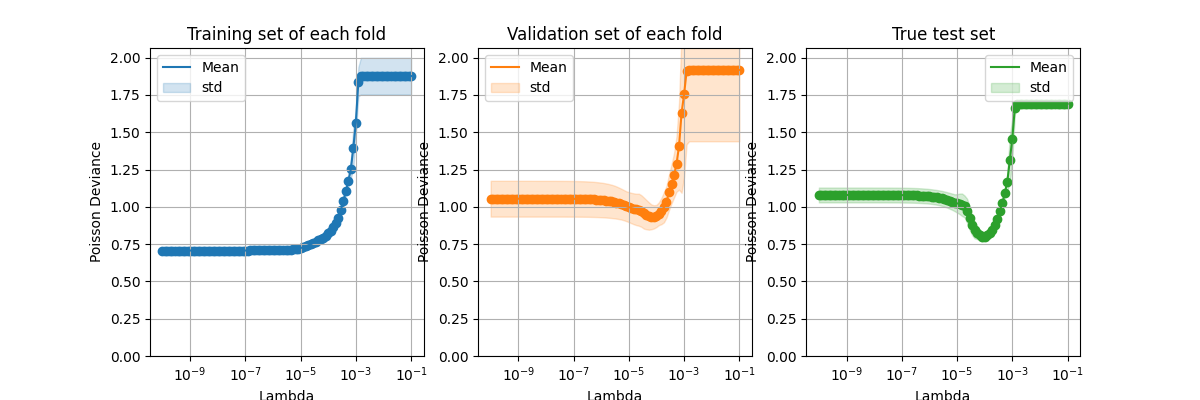
\includegraphics[width=0.75\linewidth]{extra_plots/poisson_regression_lasso_deviance_vs_lambda_no_log_transform.png}
    }
    % \hfill
    \\
    \subfloat[Log-Transformed and Normalized Data.]{
        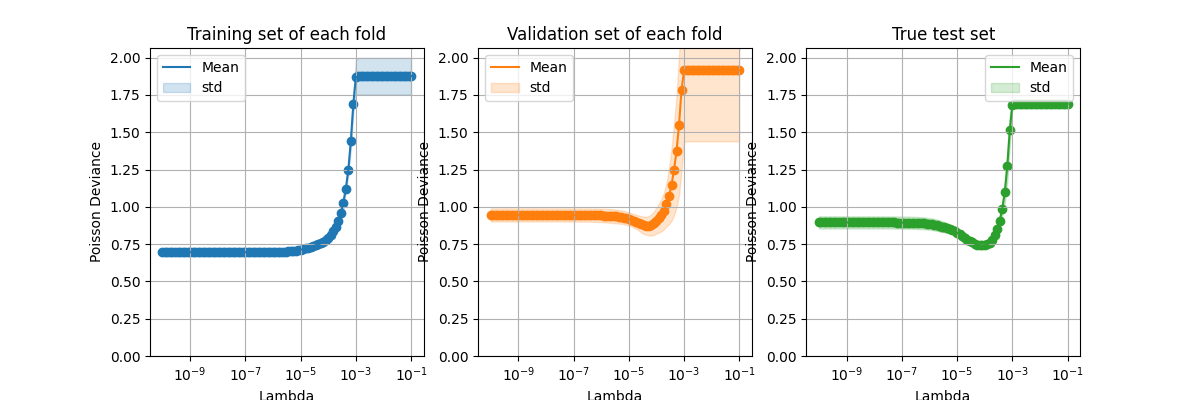
\includegraphics[width=0.75\linewidth]{extra_plots/poisson_regression_lasso_deviance_vs_lambda_log_transform.png}
    }
    \caption{The mean and standard deviation of the mean Poisson deviation score for the subset of the training set of each fold (left, blue), the hold out set for of the train set for each fold (middle, orange), and the full test set (right, green).}
    \label{fig:deviance_vs_lambda_poisson}
\end{figure}

From Figure~\ref{fig:deviance_vs_lambda_poisson}, we clearly see that lowest value for the mean Poisson deviance is convex at $\lambda \approx 10^{-4}$. In fact, we find that the best value for $\lambda$ is $1\cdot 10^{-4}$ for the just normalized data, and $8\cdot 10^{5}$ for the log-transformed data.
Using these values, we obtain the following values:
\begin{table}[htbp]
    \centering
    \begin{tabular}{l|cc}
         \toprule
         & Train & Test \\
         \midrule
         Normalized & $0.82125$ & $0.79864$ \\
         Log-Transformed \& Normalized & $\mathbf{0.77761}$ & $\mathbf{0.74252}$ \\
         \bottomrule
    \end{tabular}
    \caption{The mean Poisson deviation values for the best \textbf{Poisson regression model} obtained using \textbf{$L_1$-lasso} for the different datasets. We highlight in bold the best value of the table for each of the data splits.}
    \label{tab:deviation_poisson_l1}
\end{table}

As we can use $L_1$-regularization for feature selection, we plot the coefficients for the individual parameters over the values of $\lambda$. As we have 32 parameters in total, we add the plots in the Appendix (see Figure~\ref{fig:coefficients_lambda_normalized} and Figure~\ref{fig:coefficients_lambda_log_transformed_and_normalized}), as, while they are interesting, these plots are not at the core of this question. 

We remark that, especially in the case where we use the log-transformed data (see Figure~\ref{fig:coefficients_lambda_log_transformed_and_normalized}), all the features found by the stepwise search with the BIC score are have non-zero coefficients in the lasso regression. On the other hands, many values found by the AIC stepwise search have coefficients of zero.

However, lasso-regression, if interpreted as a feature selector, finds a different set of features as stepwise seach with BIC. For example, \texttt{numberOfVersionsUntil:} has non-zero coefficients at at the optimal value for $\lambda$, which is not included in the set of features found by any search algorithm for stepwise model search.

\subsection{Discussion}

\textbf{AIC vs BIC.}
It is clear that BIC outperforms AIC. Not only does BIC stops as soon as the test deviance increases by just looking at the training set, which is not the case for AIC.

Furthermore, while AIC keeps adding features to the model, we remark that every feature from the BIC model is included in the set of features found when using AIC (see Table~\ref{tab:coefficients_poisson_stepwise_normalized} and Table~\ref{tab:coefficients_poisson_stepwise_log_normalized}).

Therefore, together with the results from Table~\ref{tab:accuracy_logistic_stepwise}, which state that AIC overfits to the training set, whereas BIC is more robust to overfitting, we can conclude that, empirically, BIC is better at scoring models than AIC.

\textbf{Coefficients of the Model.}
Interesting, when looking at the coefficients of the learned model, we see that a very delicate balance is being optimized. For example, when looking at the coefficient for the \texttt{cbo} variable, we see that increasing it has a negative impact on the prediction, even though it has a positive coefficient (see Table~\ref{tab:coef_stepwise_logistic_normalized}).
% Comparing the coefficient of this variable to the coefficient of 
On the other hand, the oracle model for the binary classification of whether a bug is included in the code has a value around 6 times higher than in the Poisson regression model found by stepwise model selection (see Table~\ref{tab:features_coeff_logistic_normalized} in the Appendix).

This does not mean that \texttt{cbo} cannot give information on the number of bugs included in the code, but as the other variables, such as \texttt{numberOfMethodsInherited} or \texttt{weightedAgeWithRespectTo:} might better modeling capabilities of the number of bugs, removing the information of \texttt{cbo} can the Poisson regression model to better model the number of bugs.

\textbf{P-values.}
We report on the p-values of the coefficients.
While we found that AIC performs worse than BIC, we further notice that, every feature added additionally by AIC has a high p-value. 

For example, in Table~\ref{tab:coef_stepwise_logistic_normalized}, we have a p-value of 0.052 for the \texttt{noc} variable, which makes the test deviance increase. Therefore, not adding it is better.

Furthermore, using a threshold value of 0.05 or 0.01, we would reject that \texttt{noc} has an influence on the prediction of the number of bugs.

\textbf{Comparison of $L_1$-regularization and Stepwise Model Selection.}
We see that the model found by stepwise model selection with BIC as scoring outperforms the best model found by $L_1$-regularization (compare Table~\ref{tab:mean_poisson_deviation_poisson_regression_step_search} and Table~\ref{tab:deviation_poisson_l1}).

Furthermore, we see that $L_1$-regularization not only selects way more features in the model with the best value for $\lambda$, estimated on the hold out set, but out of the selected features, all of them overlap with the features found by stepwise search (see the coefficients in Figure~\ref{fig:coefficients_lambda_normalized} and Figure~\ref{fig:coefficients_lambda_log_transformed_and_normalized}).

\section{Logistic Regression}

We constructed a binary target variable \texttt{bugbin}, where $\texttt{bugbin}=1$ if $\texttt{bugs}\ge1$ and 0 otherwise. 
% A logistic regression model was fitted and forward stepwise selection using AIC was performed on the training set.
We perform the same analysis as done in the previous section, however, instead of reporting on the mean Poisson deviation, we report on the mean accuracy. 

% Due to the change in the parametrization of the model, we have to adjust our definition for $\delta_i$.

% We know from the lecture that 
% \begin{equation}
%     \frac{\mathbb{E}[y\mid x + \delta]}{\mathbb{E}[y\mid x]} \propto \exp(\beta_i \cdot \delta_i)\;.
% \end{equation}
% Therefore


\subsection{Stepwise Model Selection}

We observe the same relationship between the AIC and BIC search as in Section~\ref{sec:poisson_stepwise}.
Therefore, we will only report on the stepwise search using BIC and omit to report on the performance of the AIC search.
We plot in Table~\ref{fig:accuracy_logistic_regression} the evolution of the accuracy of the different models using stepwise search. 
We omit a detailed discussion of the plots, as we would use the same arguments denoted in Section~\ref{sec:poisson_stepwise}.

\begin{figure}[t]
    \centering
    % {\textbf{Log-Transformed \& Normalized} Data} \\
    \subfloat[Using \textbf{Normalized} Data.]{
        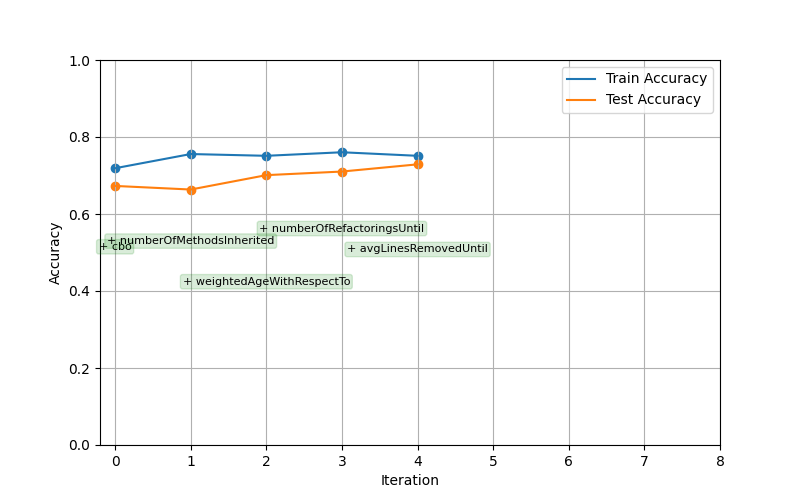
\includegraphics[width=0.45\linewidth]{extra_plots/logistic_regression_stepwise_accuracy_history_bic_no_log_transform.png}
    }
    \hfill
    \subfloat[Using \textbf{Log-Transformed \& Normalized}.]{
        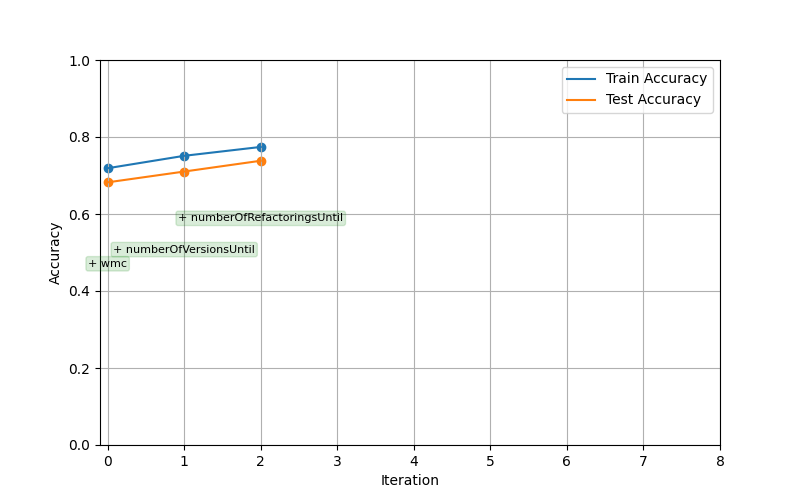
\includegraphics[width=0.45\linewidth]{extra_plots/logistic_regression_stepwise_accuracy_history_bic_log_transform.png}
    }
    \caption{Train and test deviance of the \textbf{Logistic regression} when using \textbf{stepwise model selection} with \textbf{BIC}. Note that the green boxes starts with + denote which feature has been added to the model.}
    \label{fig:accuracy_logistic_regression}
\end{figure}
We therefore obtain the following accuracies for the stepwise search:
% 0.751152, Test accuracy: 0.728972
% 0.774194, Test accuracy: 0.738318
\begin{table}[htbp]
    \centering
    \begin{tabular}{l|cc}
         \toprule
         \textbf{Set} & \textbf{Train} ($\uparrow$) & \textbf{Test} ($\uparrow$) \\
         \midrule
         Normalized & $0.751152$ & $0.728972$ \\
         Log-Transformed \& Normalized & $\mathbf{0.774194}$ & $\mathbf{0.738318}$ \\
         \bottomrule
    \end{tabular}
    \caption{The mean accuracy for the best \textbf{Logistic} regression model obtained using \textbf{stepwise model search} for the different datasets. We highlight in bold the best value of the table for each of the data splits.}
    \label{tab:accuracy_logistic_stepwise}
\end{table}

Similarly, we report on the values of the coefficients and their influence on the prediction in Table~\ref{tab:coef_stepwise_logistic_normalized} for the normalized dataset and in Table~\ref{tab:coef_stepwise_logistic_log_transform} for the log-transformed and normalized features.

% \todo[inline]{Talk about the $F_1$ metric, and false positive/false negatives.}

\begin{table}[htbp]
    \centering
    \begin{tabular}{l c c c c}
        \toprule
        \textbf{Variable} & \textbf{Coefficient} & $\frac{\mathbb{E}[y\mid x+\delta_i]}{\mathbb{E}[y\mid x]}$ & \textbf{p-value} & \textbf{95\% CI} \\
        \midrule
        Intercept & $-0.406$ & -- & $0.024$ & $[-0.759,\,-0.054]$ \\
        \texttt{cbo} & $1.289$ & $0.963$ & $<0.001$ & $[0.777,\,1.801]$ \\
        \texttt{numberOfMethodsInherited} & $0.694$ & $1.095$ & $0.012$ & $[0.153,\,1.235]$ \\
        \texttt{weightedAgeWithRespectTo:} & $0.549$ & $1.021$ & $0.004$ & $[0.178,\,0.921]$ \\
        \texttt{numberOfRefactoringsUntil:} & $-0.558$ & $3.951$ & $0.008$ & $[-0.969,\,-0.147]$ \\
        \texttt{avgLinesRemovedUntil:} & $0.728$ & $0.959$ & $0.019$ & $[0.119,\,1.337]$ \\
        \bottomrule
    \end{tabular}
    \caption{The coefficients of the Logistic regression model found using \textbf{stepwise search} with \textbf{BIC} for the \textbf{normalized} data.}
    \label{tab:coef_stepwise_logistic_normalized}
\end{table}

\begin{table}[htbp]
    \centering
    \begin{tabular}{l c c c c}
        \toprule
        \textbf{Variable} & \textbf{Coefficient} & $\frac{\mathbb{E}[y\mid x+\delta_i]}{\mathbb{E}[y\mid x]}$ & \textbf{p-value} & \textbf{95\% CI} \\
        \midrule
        Intercept & $-0.621$ & -- & $0.001$ & $[-0.974,\,-0.268]$ \\
        \texttt{wmc} & $0.986$ & -- & $<0.001$ & $[0.506,\,1.466]$ \\
        \texttt{numberOfVersionsUntil:} & $1.014$ & -- & $<0.001$ & $[0.512,\,1.517]$ \\
        \texttt{numberOfRefactoringsUntil:} & $-0.482$ & -- & $0.011$ & $[-0.853,\,-0.112]$ \\
        \bottomrule
    \end{tabular}
    \caption{The coefficients of the Logistic regression model found using \textbf{stepwise search} with \textbf{BIC} for the \textbf{log-transformed \& normalized} data.}
    \label{tab:coef_stepwise_logistic_log_transform}
\end{table}

\subsection{$L_1$-Lasso Regularization}

We run the same code as in Section~\ref{sec:l1_lasso_poisson}, namely logistic regression with 5-fold cross validation on the training set.

As shown in Figure~\ref{fig:deviance_vs_lambda_poisson}, using both datasets results in almost equal plots of the the accuracy (deviation in the Figure) when plotted against the value of $\lambda$. Therefore, we move the accuracy-vs-lambda-plot for the normalized data to the Appendix (Figure~\ref{fig:logistic_regression_lasso_deviance_vs_lambda_no_log_transform}), and report on the log-transformed and normalized data in Figure~\ref{fig:logistic_regression_lasso_deviance_vs_lambda_log_transform}. 

\begin{figure}[tp]
    \centering
    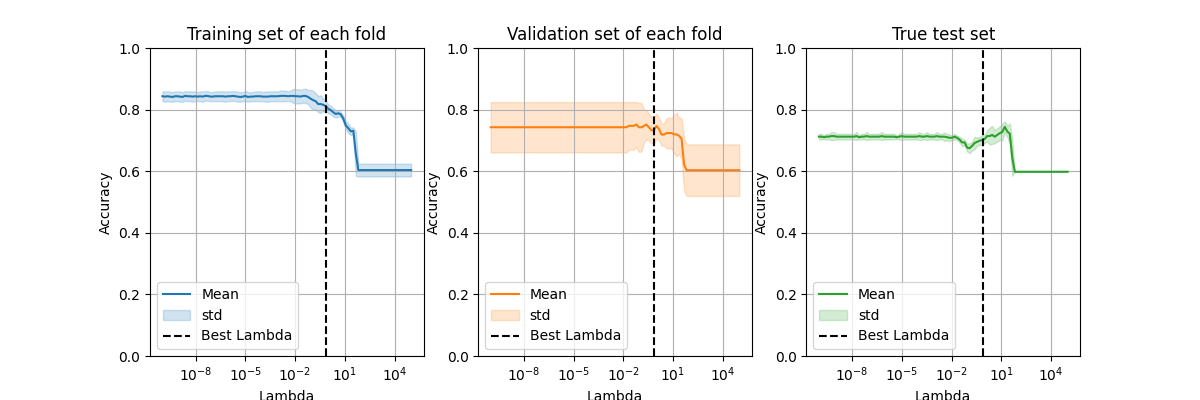
\includegraphics[width=\linewidth]{extra_plots/logistic_regression_lasso_deviance_vs_lambda_log_transform.png}
    \caption{Accuracy w.r.t. $\lambda$ for the $L_1$-lasso \textbf{logistic} regression for the log-transformed and normalized data.}
    \label{fig:logistic_regression_lasso_deviance_vs_lambda_log_transform}
\end{figure}

Surprisingly, we observe that the estimated test accuracy from the fold does not (highly) correlate with the true test set accuracy. Therefore, the value we find for best lambda, based on the estimated validation accuracy, is not at a maximum of the true test accuracy.

We again report on the optimized coefficients w.r.t. $\lambda$ in Figure~\ref{fig:logistic_regression_lasso_coefficients_log_transform} in the Appendix. We also add a table containing the coefficients of the logistic regression model learned with the best $\lambda$ value for the normalized dataset in the Appendix (Table~\ref{tab:features_coeff_logistic_normalized}).

Using the best value for $\lambda$ that we found using the hold out set of each fold, we obtain the following accuracies:
\begin{table}[htbp]
    \centering
    \begin{tabular}{l|cc}
         \toprule
         \textbf{Set} & \textbf{Train} ($\uparrow$) & \textbf{Test} ($\uparrow$) \\
         \midrule
          Normalized & $\mathbf{0.81105}$ & $\mathbf{0.74766}$ \\
         Log-Transformed \& Normalized & $0.81567$ & $0.719626$ \\
         \bottomrule
    \end{tabular}
    \caption{The mean accuracy for the best \textbf{Logistic} regression model obtained using \textbf{$L_1$-regularization} for the different datasets. We highlight in bold the best value of the table for each of the data splits.}
    \label{tab:accuracy_logistic_regression_lasso}
\end{table}

\subsection{Discussion}

First, let us discuss the results from the $L_1$-lasso regression.

\textbf{Discrepancy in Table~\ref{tab:accuracy_logistic_regression_lasso}.}
One of the most surprising results is contained in Table~\ref{tab:accuracy_logistic_regression_lasso}, where the log-transformed data got outperformed by the just normalized data. This goes goes against the trend we observed all along the report, namely that the log-transformation of the data achieves better results than the normalized results.

However, we can explain the results from Table~\ref{tab:accuracy_logistic_regression_lasso}. To this end, let us first look at the accuracy vs lambda plot of the logistic regression using the log-transformed data (Figure~\ref{fig:accuracy_logistic_regression}).
In this Figure, we can clearly see that best accuracy on the test set is obtained with $\lambda \approx 16.0$, where the mean accuracy jumps to approximately $0.7439$.
However, the highest value on the estimated accuracy on the hold out set (middle plot of the Figure) is far from the optimal $\lambda$ for achieving maximal test accuracy. 

% On the other hand, when we look at the same plots but for the just normalized data (see Figure~\ref{fig:logistic_regression_lasso_deviance_vs_lambda_no_log_transform}), we see that 
% the best lambda that was found using the hold out set matches with one of the maxima of the accuracy vs lambda curve (green curve in that Figure). 

% \todo[inline]{Add this observation to a new argument.}
% It is noteworthy to highlight that the curve on the test set (green plot) is almost maximized for any $\lambda < 10^1$. 

Therefore, while the logistic regression on the log-transformed and normalized dataset has a potential for a higher accuracy, the logistic regression on the normalized data reaches a better peak. 

\textbf{Found Features with $L_1$-Regularization.}
Let us now look at the coefficients for the best logistic regression model found when adding $L_1$-regularization on the normalized data (Table~\ref{tab:features_coeff_logistic_normalized}).

Note that interpreting the value, or even the sign, of the coefficients of a logistic regression fitted on log-transformed data is not feasible, as the impact of the value change w.r.t. the value of the input.

To gain insights from this analysis, we abstain from investigating the coefficients of the model found at $\lambda=$Best Lambda from Figure~\ref{fig:logistic_regression_lasso_deviance_vs_lambda_no_log_transform}, as we see from Figure~\ref{fig:coefficients_lambda_normalized} and Figure~\ref{fig:coefficients_lambda_log_transformed_and_normalized} that for extremely low $\lambda$ values, the variance is very high.

Furthermore, if $\lambda\approx 0$, we may risk overfitting on the training data, and therefore obtain a meaningless model.
Therefore, we cheat and use $\lambda = 1$, which maximizes the test accuracy for this case.

% We obtain the optimal test accuracy with $\lambda = 1$, and therefore  

When looking at the three most important features, we have that a coefficient for \texttt{cbo}, which denotes the Coupling Between Objects, and has a positive coefficient. This makes sense, as increasing the number of objects coupled together, if one of these objects has a bug, then all of them have a bug.
Similarly, \texttt{noc}, which stands for Number Of Children, has a strong influence on the prediction of a bug. This follows from the last argument.

Surprisingly, in this model, the number of methods (\texttt{numberOfMethods}) has a negative impact on the prediction. 

We remark that many many features that we expect to correlate with the prediction have a strong (positive or negative) influence on the prediction. For example, \texttt{numberOfRefactoringsUntil:} reduces the odds of predicting a bug by 75\% for every time a refactoring has been done. This is biased data, as code is being refactored if it contains bugs, or is prone to contain bugs.

We remark that we are unable to relate all features with respect to each other, as while the features are normalized, their value might not change the same way. For example, changing the number of lines of code will result in a much smaller difference in input (which we denote as $\Delta x$) compared to \texttt{numberOfRefactoringsUntil:} for example.

A joint analysis is way beyond the scope of this assignment, as we would need to look at the distribution of the features and the coefficients jointly, which, for 32 feature, is very vast.

\textbf{Comparison between $L_1$-Regularization and Stepwise Model Selection.}
Let us now compare the results of the $L_1$-regularization and the results from the stepwise model selection for the logistic regression.

Comparing the best found accuracies, we see that, while the log-transformed dataset outperforms the just normalized dataset when using stepwise model selection (see Table~\ref{tab:accuracy_logistic_stepwise}), the trend is reversed\footnote{See previous argument.} in the $L_1$-regularization case (see Table~\ref{tab:accuracy_logistic_regression_lasso}).

Furthermore, we see that $L_1$-regularization allows to find better performing models than stepwise model selection. 
We will discuss this in more detail in Section~\ref{sec:discussion:differences}.

The most obvious difference between both search methods is the number of features found. Whereas stepwise feature selection finds very few features (when using BIC as scoring), $L_1$ regression sets coefficients to zero only for high values of $\lambda$, where the model then degrades do to the added constraints by the regularization.

When looking at the coefficients, interestingly, the fitted models found by the stepwise model selection have drastically different coefficients for some of the parameters. For example, on the normalized data, stepwise selection finds a coefficient of $1.289$ for the \texttt{cbo} variable (see Table~\ref{tab:coef_stepwise_logistic_normalized}), in the \textit{oracle} model, we have a coefficient of $3.020$, which drastically changes the influence of the feature on the prediction. 

Investigating whether setpwise model selection could benefit from having one of the coefficient fixed from the oracle model would be an interesting future work.

\textbf{Accuracy Metric.}
While the accuracy metric is a good metric to observe how good a classification model performs, we wish to comment on the metric used.

Other popular metrics used in classification are the $F_1$ score, the selectivity, and specificity.
Which one is optimal depends on the application of the model.

We believed that, for this task, the accuracy gives us enough information to compare the different model.
However, if someone wants to, for example, develop a software that raises a warning if the probability for a bug in the function is high, then false positives are really undesired in the general case. Note that some cases have the type of error priority flipped; For example, when programming for NASA, raising a false positive is less impactful than having a false negative, and shipping code that contains a bug.

\section{Discussion --- Differences Between $L_1$-regularization and Stepwise Model Selection}

% \subsection{Differences between Stepwise Model Selection and $L_1$-Regularization}
\label{sec:discussion:differences}

Let us now comment on the differences between the two search algorithms.
A questions one might --- rightfully --- ask is \textit{which search algorithm is better?}
We believe that this question has no simple answer.

In this report alone, we have seen two cases of when one search performs better than the other; In our case, when modeling the number of bugs in the functions, we find that stepwise model selection outperforms $L_1$-regularization, whereas for predicting the existence of at least one bug, we see have found that $L_1$-regularization outperforms stepwise model selection, with even more stable accuracies.

We hypothesis that, in the case of the modeling of the number of bugs, simpler models outperform complex ones. We argue that this is due to the simpler model capturing the general trend, instead of potential noise that might correlate with the response variable in the train set but not in the test set.

If a model is dependent on a lot of variables, the probability that one of the variables changes by chance (e.g., because of noise, or hidden confounders), is very high, and therefore, the prediction might be off because of this arbitrary change.
Note that this is different from the overfitting phenomenon, which also contributes to a model having a higher number of features. However, a model having a lot of features does not necessarily overfit, whereas the probability that a model has a lot of features, given that it has overfit, is much higher.

On the other hand, for the binary prediction case, we can make use of more features, as the magnitude of the prediction is not very relevant, but rather if the prediction crosses the 0.5 boundary.
Therefore, if some noise is being added the the features, a complex model could still have the same prediction in the logistic regression case, whereas the difference to the original prediction could be quite large for the Poisson regression.

% \subsection{Finding One Bug vs Finding the Number of Bugs}

\pagebreak

% The table below shows the estimated coefficients of the selected Poisson regression model, together with standard errors, z-statistics, p-values, and 95\% confidence intervals.

% \begin{table}[h]
% \centering
% \begin{tabular}{lccccc}
% \hline
% Variable & Coefficient & Std. Error & z & p-value & 95\% CI \\
% \hline
% Intercept & -1.9665 & 0.189 & -10.388 & $<0.001$ & [-2.337, -1.595] \\
% cbo & 0.0454 & 0.004 & 12.728 & $<0.001$ & [0.038, 0.052] \\
% numberOfMethodsInherited & 0.0167 & 0.003 & 5.249 & $<0.001$ & [0.010, 0.023] \\
% weightedAgeWithRespectTo & 0.0117 & 0.002 & 5.241 & $<0.001$ & [0.007, 0.016] \\
% avgLinesAddedUntil & 0.0084 & 0.003 & 3.097 & 0.002 & [0.003, 0.014] \\
% noc & 0.1789 & 0.092 & 1.945 & 0.052 & [-0.001, 0.359] \\
% \hline
% \end{tabular}
% \end{table}

% All selected predictors have positive coefficients, indicating that higher structural complexity or more extensive code evolution is associated with a higher expected number of bugs. Most variables are statistically significant at the 5\% level, while \texttt{noc} shows a borderline effect.

% The predictive performance of the selected model was evaluated on the test set using Poisson deviance:
% \begin{itemize}
% \item \textbf{Deviance:} 0.81
% \end{itemize}

% \subsubsection{LASSO regularization}

% To model the number of bugs, we applied Poisson regression with L1 (LASSO) regularization. All predictors were standardized prior to model fitting, which is necessary for LASSO to penalize coefficients in a comparable way. The regularization parameter $\lambda$ was selected on the training set using 5-fold cross-validation, with \textbf{Poisson deviance} as the evaluation criterion.

% Cross-validation selected the following value:
% \begin{itemize}
% \item \textbf{Selected $\lambda$:} 0.166
% \end{itemize}

% Under the selected regularization strength, the LASSO Poisson model retained only a single non-zero coefficient:
% \begin{itemize}
% \item \textbf{Selected feature:} \texttt{cbo}
% \end{itemize}

% The final LASSO-selected model was evaluated on the test set:
% \begin{itemize}
% \item \textbf{Deviance:} 1.279
% \end{itemize}

% This deviance value is higher than that obtained by the stepwise Poisson model, indicating a trade-off between model simplicity and predictive accuracy.

% \subsubsection{Comparison of stepwise and LASSO}
% \begin{figure}[t]
%     \centering
%     \subfloat[Logistic regression (stepwise)]{
%         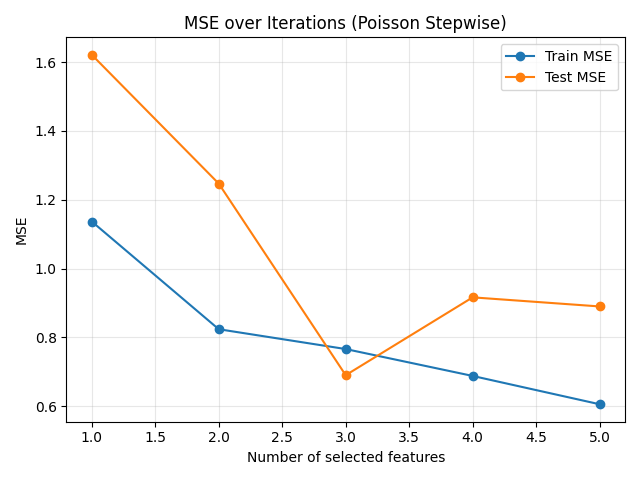
\includegraphics[width=2.5in]{MSE_PS.png}
%     }
%     \hfill
%     \subfloat[Poisson regression (stepwise)]{
%         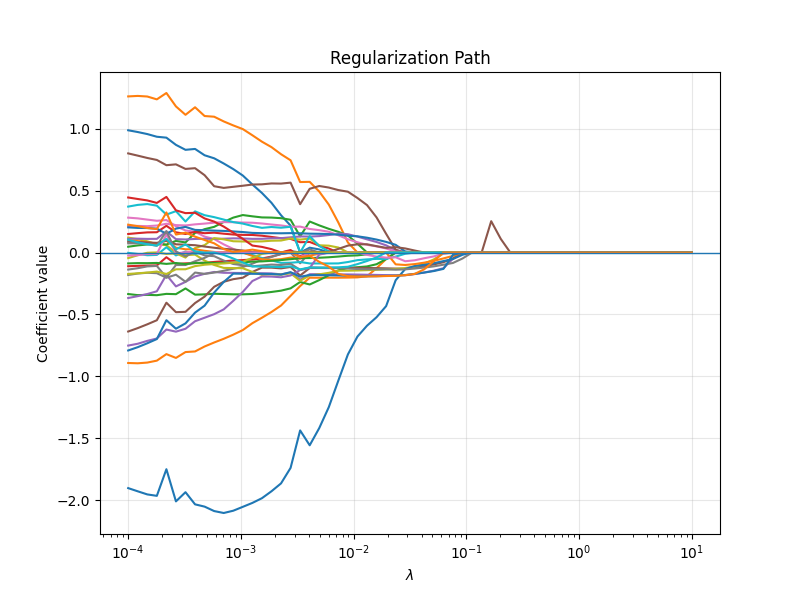
\includegraphics[width=2.5in]{reg_PL.png}
%     }
%     \caption{MSE over iterations.}
%     \label{stepwise vs LASSO}
% \end{figure}
% The stepwise-selected model includes five predictors and achieves a lower test Poisson deviance (0.81), indicating better predictive performance. In contrast, Poisson LASSO yields a much sparser model with only one predictor but results in a higher deviance (1.279). For this dataset, stepwise selection appears more suitable when predictive accuracy is the primary goal.

% As seen from Figure 3, the stepwise selection shows that Poisson regression is highly sensitive to overfitting and that adding more predictors beyond the lowest point degrades performance greatly.

%  In the LASSO regularization case, as the parameter $\lambda$ increases, most coefficients are rapidly shrunk to zero, and only few predictors remain active for moderate value of $\lambda$. Consequently, cross-validation select a strong regularization level, producing an extremely sparse model that retains only the most dominant feature.

% Comparing these two approaches, stepwise selection achieves a better balance between model complexity and predictive performance by retaining a small but informative set of predictors. On the other hand, LASSO enforces excessive sparsity, which leads to underfitting and slightly worse performance. For this dataset, stepwise selection is more suitable for Poisson regression.

% \subsection{Logistic regression}

% \subsubsection{Stepwise model selection}

% We constructed a binary target variable \texttt{bugbin}, where $\texttt{bugbin}=1$ if $\texttt{bugs}\ge1$ and 0 otherwise. A logistic regression model was fitted and forward stepwise selection using AIC was performed on the training set.

% The final model includes the following predictors:
% \begin{itemize}
% \item \texttt{cbo}, \texttt{numberOfMethodsInherited}, \texttt{weightedAgeWithRespectTo},
% \texttt{numberOfRefactoringsUntil}, \texttt{avgLinesRemovedUntil}, \texttt{noc}, \texttt{dit}
% \end{itemize}

% \begin{table}[h]
% \centering
% \begin{tabular}{lccccc}
% \hline
% Variable & Coef. & Std. Err. & z & p-value & 95\% CI \\
% \hline
% Intercept & -3.8173 & 0.629 & -6.069 & $<0.001$ & [-5.050, -2.585] \\
% cbo & 0.1191 & 0.025 & 4.845 & $<0.001$ & [0.071, 0.167] \\
% numberOfMethodsInherited & 0.0296 & 0.021 & 1.440 & 0.150 & [-0.011, 0.070] \\
% weightedAgeWithRespectTo & 0.0168 & 0.006 & 2.894 & 0.004 & [0.005, 0.028] \\
% numberOfRefactoringsUntil & -1.3044 & 0.525 & -2.486 & 0.013 & [-2.333, -0.276] \\
% avgLinesRemovedUntil & 0.0643 & 0.024 & 2.675 & 0.007 & [0.017, 0.111] \\
% noc & 0.7458 & 0.345 & 2.161 & 0.031 & [0.069, 1.422] \\
% dit & 0.8081 & 0.416 & 1.944 & 0.052 & [-0.007, 1.623] \\
% \hline
% \end{tabular}
% \end{table}

% The final model was evaluated on the test set:
% \begin{itemize}
% \item \textbf{Accuracy:} 0.720
% \end{itemize}

% \subsubsection{LASSO regularization}

% In the \texttt{sklearn} implementation, the regularization strength is controlled by parameter $C$ (with $\lambda = 1/C$). Cross-validation selected a large $C$, resulting in weak regularization and a model retaining many predictors.

% The test-set performance was:
% \begin{itemize}
% \item \textbf{Accuracy:} 0.729
% \end{itemize}

% \subsubsection{Comparison of stepwise and LASSO}
% \begin{figure}[t]
%     \centering
%     \subfloat[Logistic regression (LASSO)]{
%         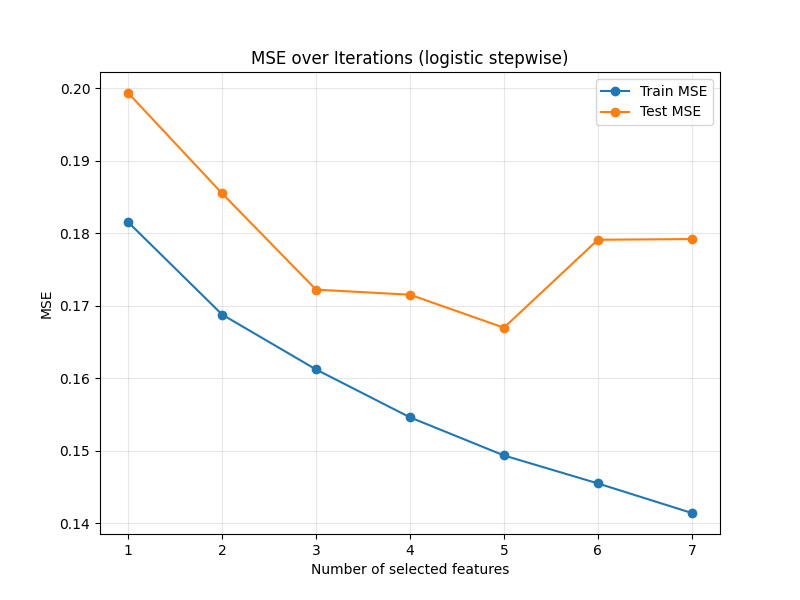
\includegraphics[width=2.5in]{MSE_LS.png}
%     }
%     \hfill
%     \subfloat[Logistic regression (stepwise)]{
%         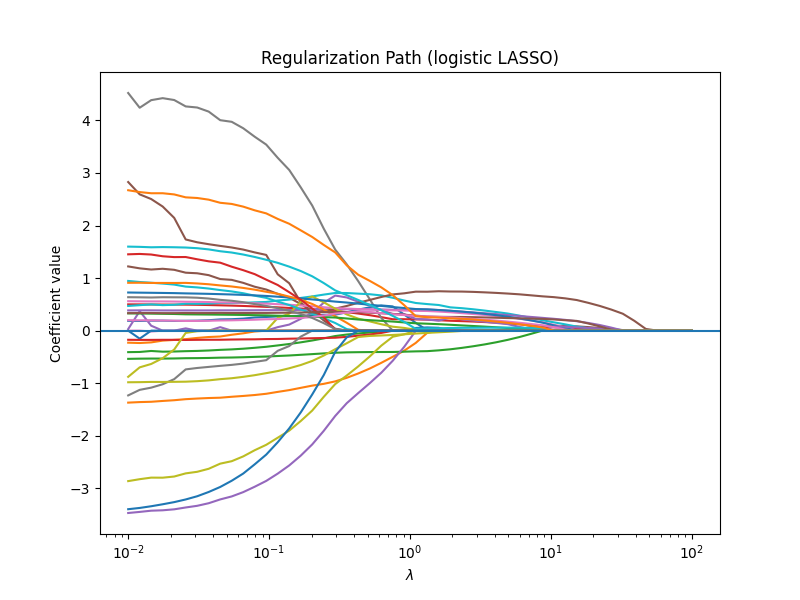
\includegraphics[width=2.5in]{reg_LL.png}
%     }
%     \caption{MSE and Regularization path.}
%     \label{fig:logistic_comparison}
% \end{figure}

% As seen from figure 4, the stepwise selection curve shows that the training MSE decreases monotonically as more features are added, while the test MSE reaches a minimum at an intermediate model size, after which increases slightly, showing stepwise selection explicitly controls overfitting by stopping the inclusion of more predictors once performance gets worse.

% On the other hand, the logistic LASSO regularization path shows a gradual decreasing of coefficients as the penalty parameter $\lambda$ increases. Rather than eliminating predictors abruptly, many coefficient remain non-zero over a wide range of $\lambda$. As a result, cross-validation selects a relatively weak regularization strength, leading to a model that retains multiple correlated predictors.

% Overall, these results indicate a key difference between these two approaches. Stepwise selection yields a more compact and easily interpretable model by directly limiting the amount of features, while LASSO controls complexity through coefficient shrinkage and achieves slightly better predictive performance by retaining a larger set of features.

% \pagebreak
